\section{Introduction}


Large language model (LLM) agents \cite{achiam2023gpt,team2023gemini,liu2024deepseek} have shown strong performance in complex task-solving settings, such as web interaction \cite{zhou2024webarena}, software engineering \cite{jimenez2024swebench}, tool use \cite{qin2024toolllm}, and long-horizon reasoning \cite{erdogan2025plan,sun2025scaling}. These settings require agents to plan, act, interpret observations, handle feedback, and recover from errors. However, when an agent fails on a task, the failure often remains an isolated event rather than a source of future improvement. Without converting failed executions into reusable lessons, agents continue to make similar mistakes in later tasks.

\begin{figure}
    \centering
    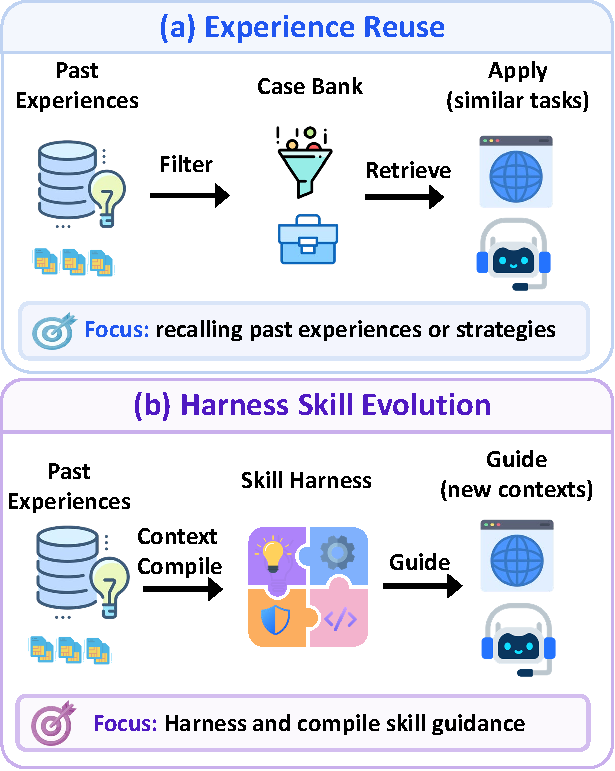
\includegraphics[width=0.7\linewidth]{figures/teaser.pdf}
\caption{
Comparison of experience reuse (retrieving past cases) and harness skill evolution (compiling experiences into reusable guidance).}
\label{fig:teaser}
\vspace{-0.5cm}
\end{figure}


\begin{figure*}
    \centering
    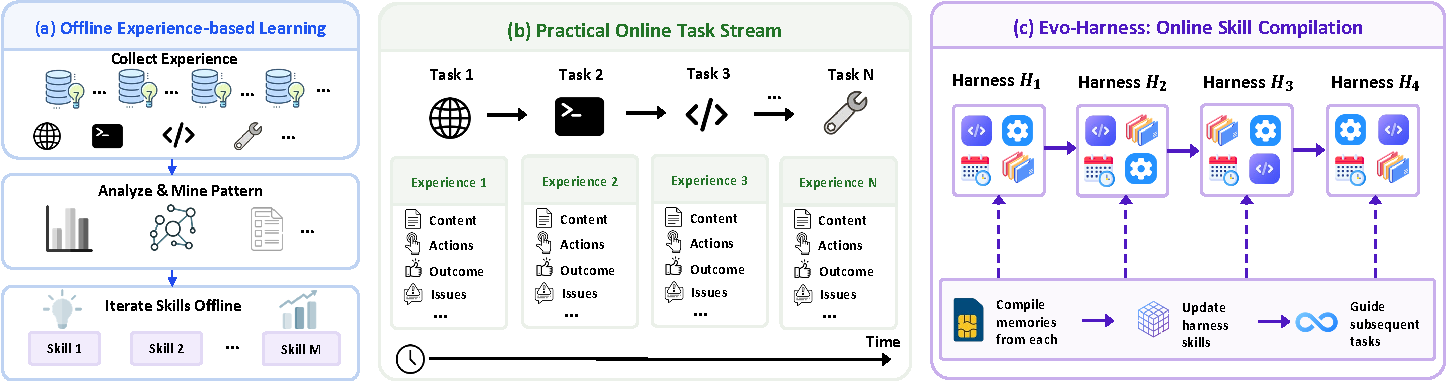
\includegraphics[width=1.03\linewidth]{figures/setting.pdf}
\caption{
Illustration of the problem setting. (a) Prior methods collect executions and mine reusable patterns offline. (b) In practical online streams, agents encounter tasks sequentially, yielding rich but one-shot execution experiences. (c) \algname{} compiles these online experiences into evolving skill harnesses for future reuse.
}
\label{fig:setting}
\vspace{-0.5cm}
\end{figure*}

Many experience-based methods~\citep{shinn2023reflexion,zhao2024expel} address this issue by learning from accumulated trajectories offline \cite{lee2026meta,ni2026trace2skill}, utilizing media such as reflection \citep{shinn2023reflexion,qiu2026autorefine}, memory \citep{zhong2024memorybank,chhikara2025mem0,xu2025mem}, and skills \citep{zhang2026memskill,xia2026skillrl,jiang2026xskill,yang2026autoskill}. However, in realistic settings, agents continuously encounter novel tasks and contexts, and each completed execution typically offers only a one-shot opportunity to improve future behavior. Furthermore, real executions produce rich but highly noisy contexts, entangling useful lessons with task-specific details, partial failures, and incidental tool traces.

Critically, prior methods often fail to rigorously validate their effectiveness under these realistic constraints, nor do they systematically isolate the underlying drivers of agent improvement. To navigate such a one-shot, complex learning environment, relying on the simple retrieval of past experiences falls short. Instead, agents need to actively compile raw execution contexts into reusable skill guidance for novel tasks, as contrasted in Figure~\ref{fig:teaser}.

Building on this view, we formulate \emph{online harness learning}, where a frozen agent improves by incrementally updating a structured, external harness across sequential tasks. To cope with the continuous influx of novel tasks, this harness acts as a self-evolving learning medium that progressively distills executions into actionable guidance for the future. An overview of this practical setting, compared to standard offline learning, is illustrated in Figure~\ref{fig:setting}.

To operationalize this formulation and enable a systematic study of continuous self-improvement, we introduce \emph{Evo-Harness}. We instantiate the harness within this framework using skills. Skills act as a natural medium for realistic task executions because they can integrate diverse learning signals, such as failures, feedback, constraints, and operational procedures, into structured knowledge that shapes future planning and recovery. At the core of \emph{Evo-Harness} is \emph{context-to-harness skill compilation}, which converts individual execution contexts into reusable skill harness updates. Specifically, our compilation process uses a \emph{solver} to reflect on contexts and propose candidate skills, and an \emph{evolver} to update the existing harness. \emph{General} skills capture transferable cross-task patterns, while \emph{topic} skills capture localized operational knowledge. This dual design preserves critical learning signals while filtering out trajectory-level noise.

We evaluate Evo-Harness across five realistic benchmarks (TerminalBench2, SWE-bench, CL-Bench, $\tau$-bench, and WebArena-Infinity) under a sequential continuous learning setup. Beyond demonstrating performance gains, our primary focus is systematically investigating the core drivers of self-improvement. By analyzing how evolver designs, feedback types, and transfer settings dictate performance, our study treats the skill harness as an interpretable object for understanding how frozen LLM agents learn on the fly.


Our contributions are summarized as follows:
\begin{itemize}[itemsep=0pt,topsep=2pt,leftmargin=*]
    \item \textbf{Online harness learning.}
    We formulate a setting where frozen agents improve over sequential task streams by incrementally updating a reusable external harness instead of model parameters.
    
    \item \textbf{Context-to-harness skill compilation.}
    We introduce a mechanism that compiles single-shot execution contexts into actionable general and topic-level skill updates.
    
    \item \textbf{Systematic analysis of harness evolution.}
    We isolate how evolver designs, feedback types, and transfer settings impact continuous self-improvement. Evaluated across five complex benchmarks, \algname{} consistently outperforms existing experience-based methods.
\end{itemize}
